\chapter{Introduction}\label{chap:chap0}

\epigraph{It's difficult to be rigorous about whether a machine really
  ``knows'', ``thinks'', etc., because we're hard put to define these
  things. We understand human mental processes only slightly better
  than a fish understands swimming.}{John McCarthy}
\clearpage

\section{Les enjeux de la robotique}

\subsection{État de la robotique en 2012}

\lettrine[lines=2, lraise=0.1, nindent=0em, slope=-.5em]%
{I}{l} a beaucoup été écrit, et il a beaucoup été dit sur la robotique. On
annonce depuis plusieurs décennies son avènement prochain et pourtant
elle peine à s'imposer dans nos quotidiens. Il y a pourtant des
raisons d'espérer! Le rapport PIPAME sur Le développement industriel
futur de la robotique personnelle et de service en France
\citep{12erdyn} estime qu'en 2015, au niveau mondial, le marché de la
robotique de service personnelle représentera 8 milliards de dollars
tandis que le marché de la robotique de service industrielle
représentera, quant à elle, 18 milliards de dollars. Les gouvernements
investissent largement dans les programmes de recherche en Europe et
aux États-Unis -- la \emph{National Robotics Initiative}, par exemple,
est un programme de 70 millions de dollars pour la coopération
humain/robot --. Une explication de l'intérêt grandissant des pouvoirs
publics pour ces technologies est la nécessité, pour les pays
développés, de trouver de nouveaux axes de croissance et de lutter
contre la délocalisation. L'automatisation de l'industrie représente
une stratégie, notamment mise en avant par le Symop -- Syndicat des
Entreprises de Technologies de Production -- au travers de leur site
``Robotcaliser''\footnote{Site officiel:
  \url{http://www.robotcaliser.com/}}. Cette large poussée en avant
s'observe également par les compagnies telles iRobot qui ont réussi à
faire un pas vers l'entrée de la robotique dans nos quotidiens. Leur
robot aspirateur Roomba est un des exemples de produits robotiques
grand public ayant trouvé son marché et commençant à concurrencer
sérieusement les aspirateurs non autonome.


Une autre application susceptible d'accéder au stade industriel dans
la prochaine décennie est la voiture autonome. Les défis proposés par
la DARPA -- Defense Advanced Research Projects Agency -- fournissent
un bon aperçu de la vitesse à laquelle la robotique peut progresser:
en 2004, aucune voiture n'a réussi à réalise plus de 11,78 km sur les
240 km que comptait la course. En 2005, cinq véhicules ont terminé la
course dans sa totalité, l'équipe la plus rapide étant celle de
Stanford avec un temps de parcours total de 6 heures et 54 minutes. En
2007, le défi a sensiblement changé puisque l'objectif était de
réaliser 96 km de navigation autonome, en ville, tout en respectant le
Code de la route et en prenant en compte la circulation extérieure:
piétons et autres voitures non automatiques. Un aboutissement a
également été, en 2012, la possibilité pour un aveugle d'être
conduit par une voiture automatique conçue par Google de son domicile
à un commerce local. Dans un domaine très lié à celui de la robotique,
celui des capteurs, l'année 2010 a été l'année de la
Kinect\index{Kinect (Microsoft)}. Ce capteur destiné à la console de
jeux Xbox 360 de Microsoft filme l'utilisateur tout en construisant
simultanément une carte de profondeur dense. Cet accessoire permet de
jouer aux jeux sans manette, en utilisant son propre corps pour
interagir avec la console. La conception de ce capteur a donné à la
communauté robotique un moyen peu onéreux -- 150 euros environ -- de
percevoir l'environnement en 3D. Un capteur aux capacités proches,
mais dédié à la recherche scientifique tel que le Swiss
Ranger\index{Swiss Ranger} est actuellement vendu pour plusieurs
milliers d'euros selon les modèles. Un tel changement dans l'échelle
des prix, rendu possible par une industrialisation de masse affecte
évidemment de manière indirecte le domaine.


\begin{figure}
  \begin{center}
    \includegraphics[width=\linewidth]{src/chap0-introduction/pr2.jpg}
  \end{center}
  \caption{Le robot PR2\index{PR2 (robot)} de la société Willow Garage. \label{fig:pr2}}
\end{figure}


Le gain en maturité du marché de la robotique se voit également dans
les laboratoires de recherche. Il y a encore dix ans, les robots
présents dans les laboratoires étant dans la quasi-totalité des cas
réalisés par les chercheurs sur place. Cela nécessitait des
compétences très étendues de la mécanique à l'électronique afin de
réaliser une intégration correcte des différents composants. Comme
tous les prototypes, ces robots étaient généralement peu fiables et
difficiles à utiliser. Depuis quelques années la tendance s'inverse et
les robots des laboratoire de recherche sont en train de devenir des
``produits finis'' manufacturés par quelques grands groupes
industriels tel que Kuka en Allemagne ou Kawada Industries au Japon ou
bien encore par des start-ups innovantes comme Willow Garage aux
États-Unis. Ce dernier exemple est révélateur du niveau de qualité
atteint par la robotique mobile à roue: le robot PR2, voire
\autoref{fig:pr2}, est certes cher -- 400 000 dollars! -- mais
comporte 7 caméras, un projecteur de lumière structurée, deux bras
perfectionnés, deux capteurs lasers permettant de cartographier
l'environnement, deux ordinateurs puissants et un ensemble de roues
motorisées permettant un déplacement omnidirectionnel. Un tel robot
arrive avec un ensemble de logiciels préinstallés permettant de
s'abstraire d'une large partie des problèmes robotiques ``de base'':
calibration des caméras, cartographie et navigation automatique,
génération de trajectoires afin de réaliser des scénarii type ``pick
and place'' où le robot doit prendre un objet et le déposer
ailleurs. Posséder un robot ayant un tel niveau de fonctionnalité dès
``qu'on le sort de sa boîte'' est un signe important et n'était pas
envisageable ne serait ce qu'il y a cinq ans. De plus, comme tout
produit construit en série, aussi petite soit-elle, ce robot, le
PR2\index{PR2 (robot)}, bénéficie de tests de fiabilité, d'une
documentation importante et d'une véritable assitance technique. Le
gain en productivité pour les chercheurs est réel et dès lors, il est
clair que la robotique mobile est en train de passer d'une activité de
recherche composée de prototypes à une activité industrielle
structurée par des acteurs imposant leur plate-forme logicielle et
matérielle.



\subsection{L'enfance de l'Art de la robotique humanoïde}


La robotique humanoïde, quant à elle, se démarque des autres robots
mentionnés plus tôt. Alors que les drones et autres robots mobiles
commencent à s'enorgueillir d'une qualité quasi industrielle, les
robots humanoïdes sont encore au stade de l'enfance. Tant la
conception mécanique, que les systèmes de contrôle ou bien encore des
systèmes de perception adaptés restent à améliorer pour arriver à
obtenir un robot pouvant évoluer de manière réellement
autonome. Poussées par la fiction d'une part et la comparaison à
l'homme d'autre part, les attentes pour ce type de technologies sont
importantes alors que les résultats pratiques restent difficiles à
obtenir. L'instabilité inhérente à la locomotion bipède et le nombre
important de degrés de liberté -- de possibilité de mouvement --
rendent les schémas de contrôle particulièrement difficiles à
concevoir. De nombreuses questions restent ouvertes telles que:
comment réagir à une perturbation extérieure pendant la marche -- le
robot glisse ou bien il est poussé --? Quelle conception mécanique
permettrait d'assurer à la fois une résistance aux impacts, pour la
course, le saut, mais également une grande vélocité pour d'autres
usages, comme taper dans un ballon? Quels sont les modèles optimaux
pour générer des mouvements stables le plus rapidement possible?
Répondre à toutes ces questions, qui ne sont pas uniquement des
questions algorithmiques, est primordial pour arriver à concevoir un
robot humanoïde utile et autonome.

\begin{figure}
  \begin{center}
    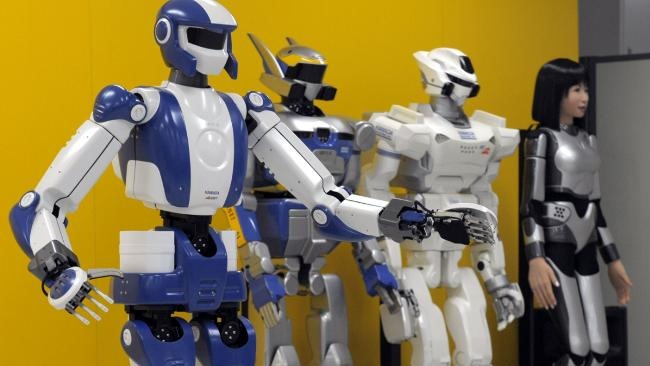
\includegraphics[width=\linewidth]{src/chap0-introduction/hrp_family.jpg}
  \end{center}
  \caption{Les robots HRP-4, HRP-2, HRP-3 et HRP-4c (de gauche à
    droite). \label{fig:hrpfamily}}
\end{figure}

Les robots humanoïdes se divisent en deux catégories: ceux de petite
taille comme le robot Nao d'Aldebaran Robotics \citep{wikipedia.nao}
et les humanoïdes de grande taille tels que ceux développés dans le
cadre du projet HRP ou bien encore par les sociétés avec le robot
Partner ou Honda avec robot Asimo. Les problématiques posées par les
deux types d'humanoïde sont assez différentes. Les robots de petite
taille utilisent des actionneurs moins puissants, de qualité moindre,
sont d'une conception moins précise par ils utilisent souvent des
squelettes en plastique plutôt qu'en métal pour des questions de
coût. Leurs capacités de calcul sont également souvent très limitées
au point qu'un ordinateur externe est souvent nécessaire pour les
commander. Les enjeux sont donc ici comment limiter les calculs
nécessaires à bord du robot étant donné les fortes contraintes sur la
capacité de calcul, comment prendre en considération les imperfections
dans la modélisation du robot, la flexibilité de ses différentes
parties ou bien encore la mauvaise précision de ses
actionneurs. L'objectif étant de fournir à moyen terme un robot
compagnon réalisant des tâches simples comme jouer avec un humain ou
fournir des services simples comme la télésurveillance. Les capacités
de manipulation de ces humanoïdes sont, à l'heure actuelle, très
limitées, voire inexisantes.


Au contraire, les grands humanoïdes sont extrêmement onéreux et
composés de pièces usinées très précisément et d'actionneurs
extrêmement performants. De ce fait, les problèmes d'identification de
modèles ne se posent qu'à la marge et le mouvement réel du robot est
très proche de sa simulation faisant l'hypothèse de mouvements de
corps rigides. Les capacités de calcul sont également plus importantes
bien qu'inférieures à ce que l'on peut trouver dans un robot mobile où
un poids important ne pose pas de problème particulier. Selon les
modèles, ces robots peuvent réaliser des tâches de manipulation
complexe. Les défis posés par ces robots sont différents: ils sont
plus lourds, plus grands et donc toute chute leur est généralement
fatale. La commande à gain fort courante sur ce type de système rend
également le comportement du système potentiellement dangereux: pour
atteindre sa consigne, le robot aura tendance à appliquer le couple
maximal de ses actionneurs, quitte à s'endommager lui-même ou à
blesser un humain se trouvant à proximité. Ils restent donc, à l'heure
actuelle, des outils de recherches dangereux impropres à une
utilisation à proximité d'humains.


\subsection{Le projet japonais HRP}


\begin{figure}
  \begin{center}
    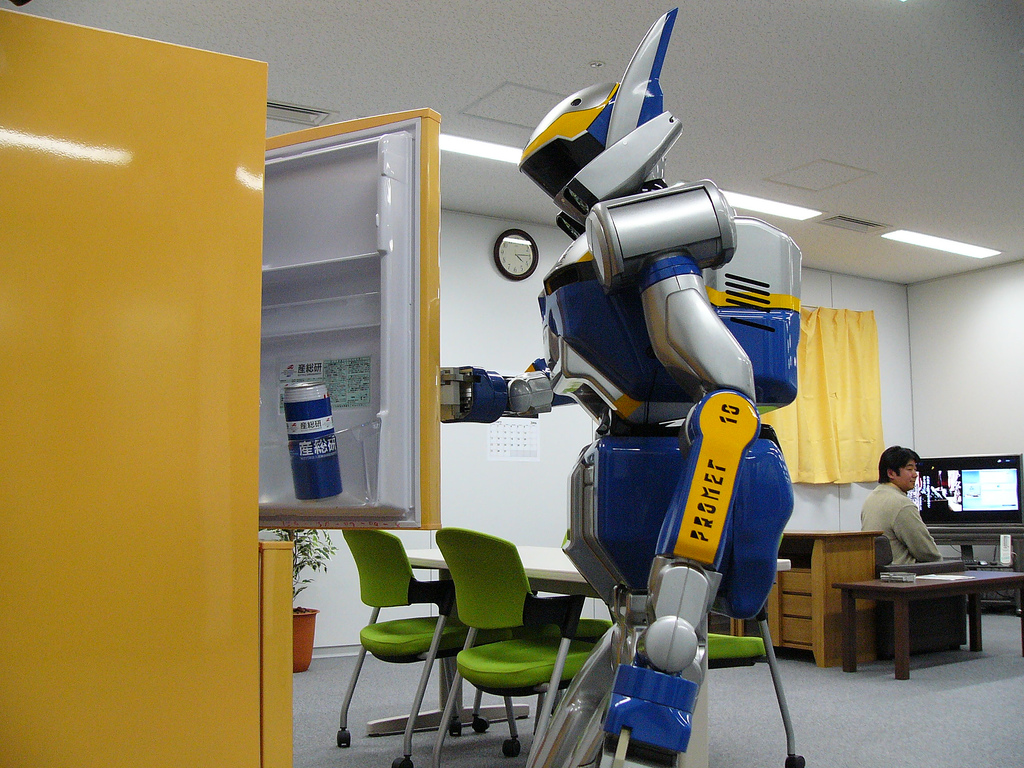
\includegraphics[width=\linewidth]{src/chap0-introduction/hrp2.jpg}
  \end{center}
  \caption{Le robot HRP-2\index{HRP-2} réalisant une tâche de
    manipulation. \label{fig:hrp2}}
\end{figure}


La totalité des recherches effectuées durant cette thèse et qui sont
décrites ici ont été validées sur la plate-forme robotique HRP-2
\citep{04kaneko.icra} du LAAS. Une version alternative est illustré
par la \autoref{fig:hrp2}. Le robot humanoïde HRP-2 ``Promet'' est un
robot humanoïde japonais mesurant 154cm et pesant 58kg. Il dispose de
deux jambes à six degrés de liberté, de deux bras à six degrés et de
deux mains à un degré de liberté commandant l'ouverture de la pince
composant chaque préhenseur. Deux degrés de liberté sont affectés au
mouvement de la tête et les deux derniers actionnent l'articulation du
torse du robot. Cette dernière étant une caractéristique unique de
cette plate-forme. Le nombre total de degrés de liberté du système est
donc de 30. Les capteurs de ce robot comprennent quatre capteurs de
force six-axes aux chevilles et au poignet, ainsi qu'une centrale
inertielle dans le torse mesurant la vitesse angulaire et
l'accélération linéaire du torse. Un système de caméras composé de
deux paires stéréo situées dans la tête est également présent. Une
première paire possède des objectifs grand-angles permettant de
percevoir une large portion de l'environnement entourant le robot
tandis que la seconde a un angle de vue plus étroit, permettant une
bonne précision lors de la manipulation. Ce robot dispose d'un système
absorbant les chocs dans chaque cheville afin de protéger la mécanique
des impacts réalisés pendant la marche. Les traitements embarqués sont
réalisés par deux ordinateurs reliés entre eux par un réseau
Ethernet. La connexion avec l'extérieur est assurée par un point
d'accès WiFi.


Ce robot conçu en 1998 a été suivi du robot HRP-3 en 2007, du robot
HRP-4C en 2009 et du robot HRP-4 en 2010. HRP-3 s'est démarqué en
étant le premier robot humanoïde résistant à l'eau ouvrant la porte à
une utilisation de ces robots en extérieur. HRP-4c est un gynoïde,
c'est-à-dire un robot humanoïde possédant l'apparence d'une femme. Les
applications ciblent le domaine du mannequinat et du divertissement
plus généralement. Le dernier robot de la série, HRP-4 est, quant à
lui, plus léger tout en conservant sept degrés de liberté pour les
bras et deux degrés de liberté pour les mains. Les différents modèles
sont illustrés par la \autoref{fig:hrpfamily}.


\section[Contributions]{Contributions, de la génération de mouvements à leur exécution}


Le maître mot de ces trois ans et demi est finalement, et cela ne peut
que se ressentir à la lecture de ce manuscrit, la polyvalence. Comme
dans toute thèse expérimentale, il a été nécessaire de tenter de
mettre en pratique des idées, de A à Z. C'est à la fois formateur et
passionnant, mais m'a conduit à utiliser de très nombreux outils,
algorithmes de l'État de l'Art et à les comprendre afin de pouvoir les
intégrer à l'approche que j'ai souhaité développer. Le travail réalisé
étant principalement de faire communiquer les idées entre elles:
comment un algorithme de vision peut-il servir la commande? Comment
les données capteur peuvent-elles être utilisées par différents
composants?  Autant de questions qui, en terme d'ingénierie
logicielle, consistent à lier des boîtes entre elles, encapsulant
autant d'algorithmes et de stratégies de décision différentes. Il est
toutefois difficile d'argumenter sur la pertinence des ``flèches''
sans expliquer au préalable ce que contiennent les ``boîtes'',
d'autant que si certaines techniques sont classiques en robotique,
d'autres sont issues des recherches du groupe GEPETTO et ne peuvent
être considérées comme allant de soi. Le choix réalisé lors de la
rédaction a donc été d'expliquer progressivement comment réaliser des
scénarii complexes avec un robot humanoïde, de la théorie, à la
pratique, mes contributions se situant davantage dans ce spectre. Le
premier chapitre de ce manuscrit traite d'un problème particulier
abordé dans le cadre de cette thèse: la représentation informatique
des problèmes d'optimisation numérique. Ce problème peut sembler
distinct de la robotique humanoïde, mais les techniques d'optimisation
sont devenues un socle supportant tant d'algorithmes utiles qu'on ne
peut pas éluder la question de la représentation de ces
problèmes. L'objectif ici est de s'appuyer sur les caractéristiques
des langages de programmation modernes, tel que le C++ afin de pouvoir
définir un problème d'optimisation une fois puis de pouvoir le
transmettre à différents solveurs de façon transparente. Une
application robotique simple valide cette approche, mais la
contribution majeure reste la formulation et la modélisation
informatique du problème. Le second chapitre explique pas à pas les
techniques de génération de mouvement et d'exécution sur le robot. Ces
techniques font partie de l'État de l'Art et il n'y a pas d'apport
original à ce niveau. Cependant, le contrôleur construit sur ces
techniques et permettant de suivre des trajectoires tout en
incorporant les données capteur est un travail totalement original et
sur lequel, à notre connaissance, aucun article antérieur n'a été
publié. Le troisième chapitre est divisé en deux: tout d'abord la
description informatique d'une pile de tâches asservie est un apport
original. La suite du chapitre est dédiée à la localisation utilisant
la vision sur un robot humanoïde. Cette partie n'est pas nouvelle en
soi, car des résultats similaires ont déjà été publiés dans ce
domaine, mais l'intégration de la localisation au schéma de contrôle
proposé dans le \autoref{chap:suivi} est un travail original. Le
dernier chapitre traite de l'intégration des différents composants sur
notre plate-forme robotique. Dans ce chapitre, la totalité des
algorithmes proposés font, soit partie de l'État de l'Art, soit ont été
conçus par d'autres équipes partenaires du LAAS, notamment l'équipe
\mbox{LAGADIC} de l'IRISA à Rennes. L'apport original de cette partie
consiste à démontrer comment on peut construire une architecture
robotique complète en utilisant des algorithmes existant afin
d'atteindre des comportements de plus haut niveau.
